\documentclass[a4paper,11pt]{article}


\usepackage{geometry} % for making easy changes to page layout
\geometry{body={15cm,24cm}} % change height and width of main text
\usepackage{yhmath}

\usepackage{parskip} % for blank lines between paragraphs 
\usepackage{bbm}

\usepackage{amsmath,amssymb} % for serious mathematics, such as \begin{align*} etc

\usepackage{graphicx} % for \includegraphics[width = 1\textwidth]{} etc
\usepackage{booktabs}

\title{GLM Practical}
\author{P806}
\date{7 Decembre 2022}

\begin{document}

\maketitle

\section{Introduction}
The presented dataset consists 5190 responses to a survey about doctor visits. For each response, the number of doctor visits in the two weeks before the survey is the response variable, and information about the age, income, insurance, and chronic diseases is recorded. Hence the design of the dataset is
\begin{align*}
\centering
\mathbf{x}  & \longmapsto y \\
\mathbf{x} &= (\text{Age, Gender, Income, Type of Insurance, Chronic Condition}) \\
 &= (x^{(a)}, x^{(g)}, x^{(i)}, x^{(t)}, x^{(c)}) \\
y &= \text{Number of Doctor Visits in preceding two weeks}
\end{align*}
$a$ and $i$, the age and the income of survey respondents, are real numbers, while $t$ and $c$ are categorical variables.

Note that in the raw dataset, there is no column on insurance type, but the insurance type is constructed from the columns \texttt{private, freepoor, freerepat}. Those columns are binary indicator variables for the three insurance types, and they are never all \texttt{1} for any sample. So, we can just create a variable \texttt{insurance} that is a categorical variable and has four different possible values: \texttt{private, freepoor, freerepat}, and \texttt{normal}. $\texttt{insurance} = \texttt{normal}$  if \texttt{private, freepoor, freerepat} are all $0$ in the original dataset.

Similarly, there is not actually a \texttt{gender} variable in the dataset, but only binary indicator if the respondent was female or not. For simplicity, we converted that indicator into a categorical variable that has the values \texttt{male} and \texttt{female}.
\begin{figure}[h]
	\centering
	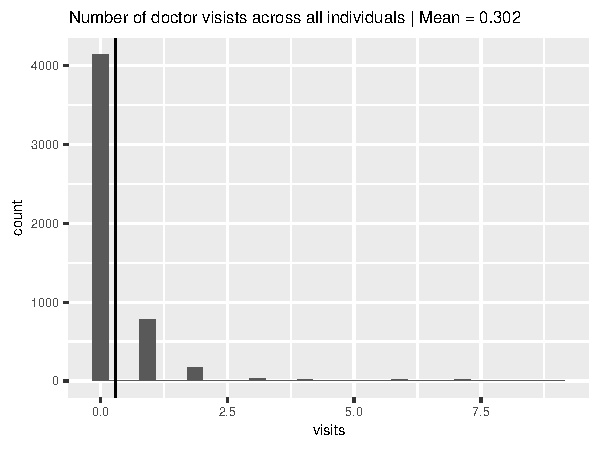
\includegraphics{../plots/histogram_of_visits.pdf}
	\caption{Histogram of entire dataset}
	\label{fig:hist_all}
\end{figure}

\section{Data Exploration}
First, looking at figure \ref{fig:hist_all}, we see that a large majority of the survey answers are $0$. The mean response is $0.302$. Considering that we are counting occurrences of events and the large zero-count, a Poisson model lends itself as a good model to fit to the data. The model will help us understand the relationship of the different features of the $\mathbf{x_i}$ and the count of doctor visits, $y_i$.

Figure \ref{fig:hist_insurances} gives a first glimpse into that relationship. We see the same plot as in figure \ref{fig:hist_all}, but for the dataset split by the type of insurance the survey respondents had. We see that the type of insurance has some influence of the mean number of visits to the doctor. In particular, people with free government insurance due to old age, disability, or veteran status, i.e., $x^{(t)} = \texttt{freerepat}$ have a much higher mean number of doctor visits than people with other type of insurance. 

\begin{figure}[h]
	\centering
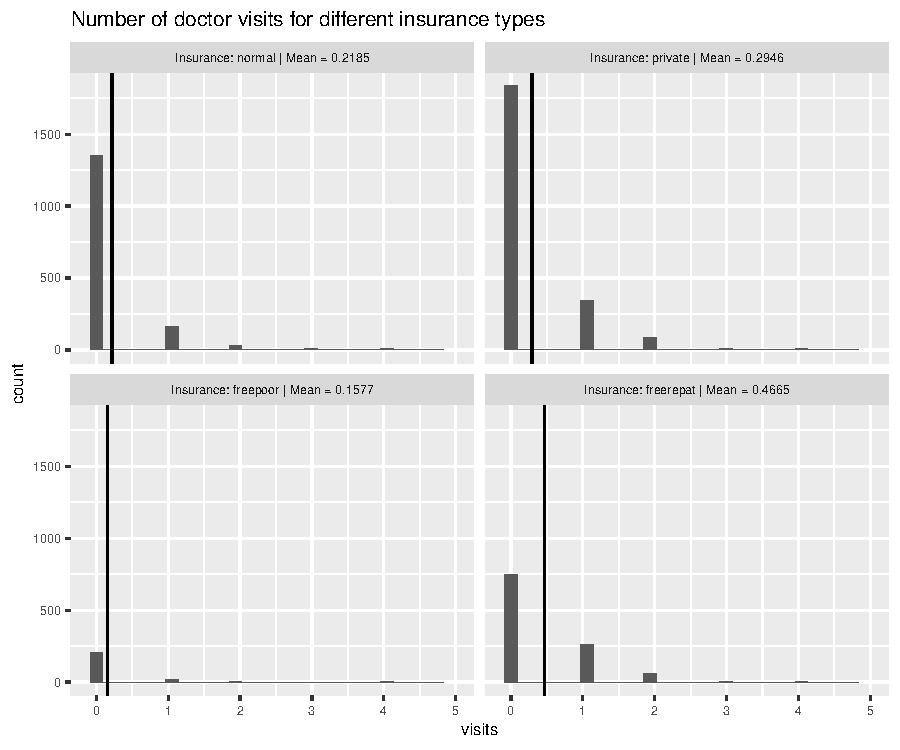
\includegraphics{../plots/histograms_of_insurances.pdf}
		\caption{Histogram of data split by type of insurance}
			\label{fig:hist_insurances}
\end{figure}

This is supported by table \ref{tab:stats_fine}. We see that both for male and female respondents, the mean number of doctor visits of respondents with the \texttt{freerepat} insurance is the highest. Interestingly, the number of doctor visits from those patients also has the highest variance. In general, we see that the variance of doctor visits increases with increasing mean, albeit that the data from female respondents has in general higher variance.

\input{../report/descriptive_stats_fine.txt}

Table \ref{tab:stats_coarse} shows the effect of the gender on doctor visits in more detail. We see again that females have a higher mean number of visits and variance of visits. But in this table, it comes apparent that this might actually be the case because the sample includes women of a higher age, on average.

In order to understand if the age has an influence on the number of doctor visits, we refer to figure \ref{fig:scatter_income_and_age}. There, we see nicely how the mean number of doctor visits \emph{decreases} with increasing age and \emph{increases} with increasing age. We might thus postulate the hypotheses that the mean number of doctor visits depends strongly on age and income. We shall further investigate this hypothesis in the next section.

\input{../report/descriptive_stats_coarse.txt}

\begin{figure}[h]
	\centering
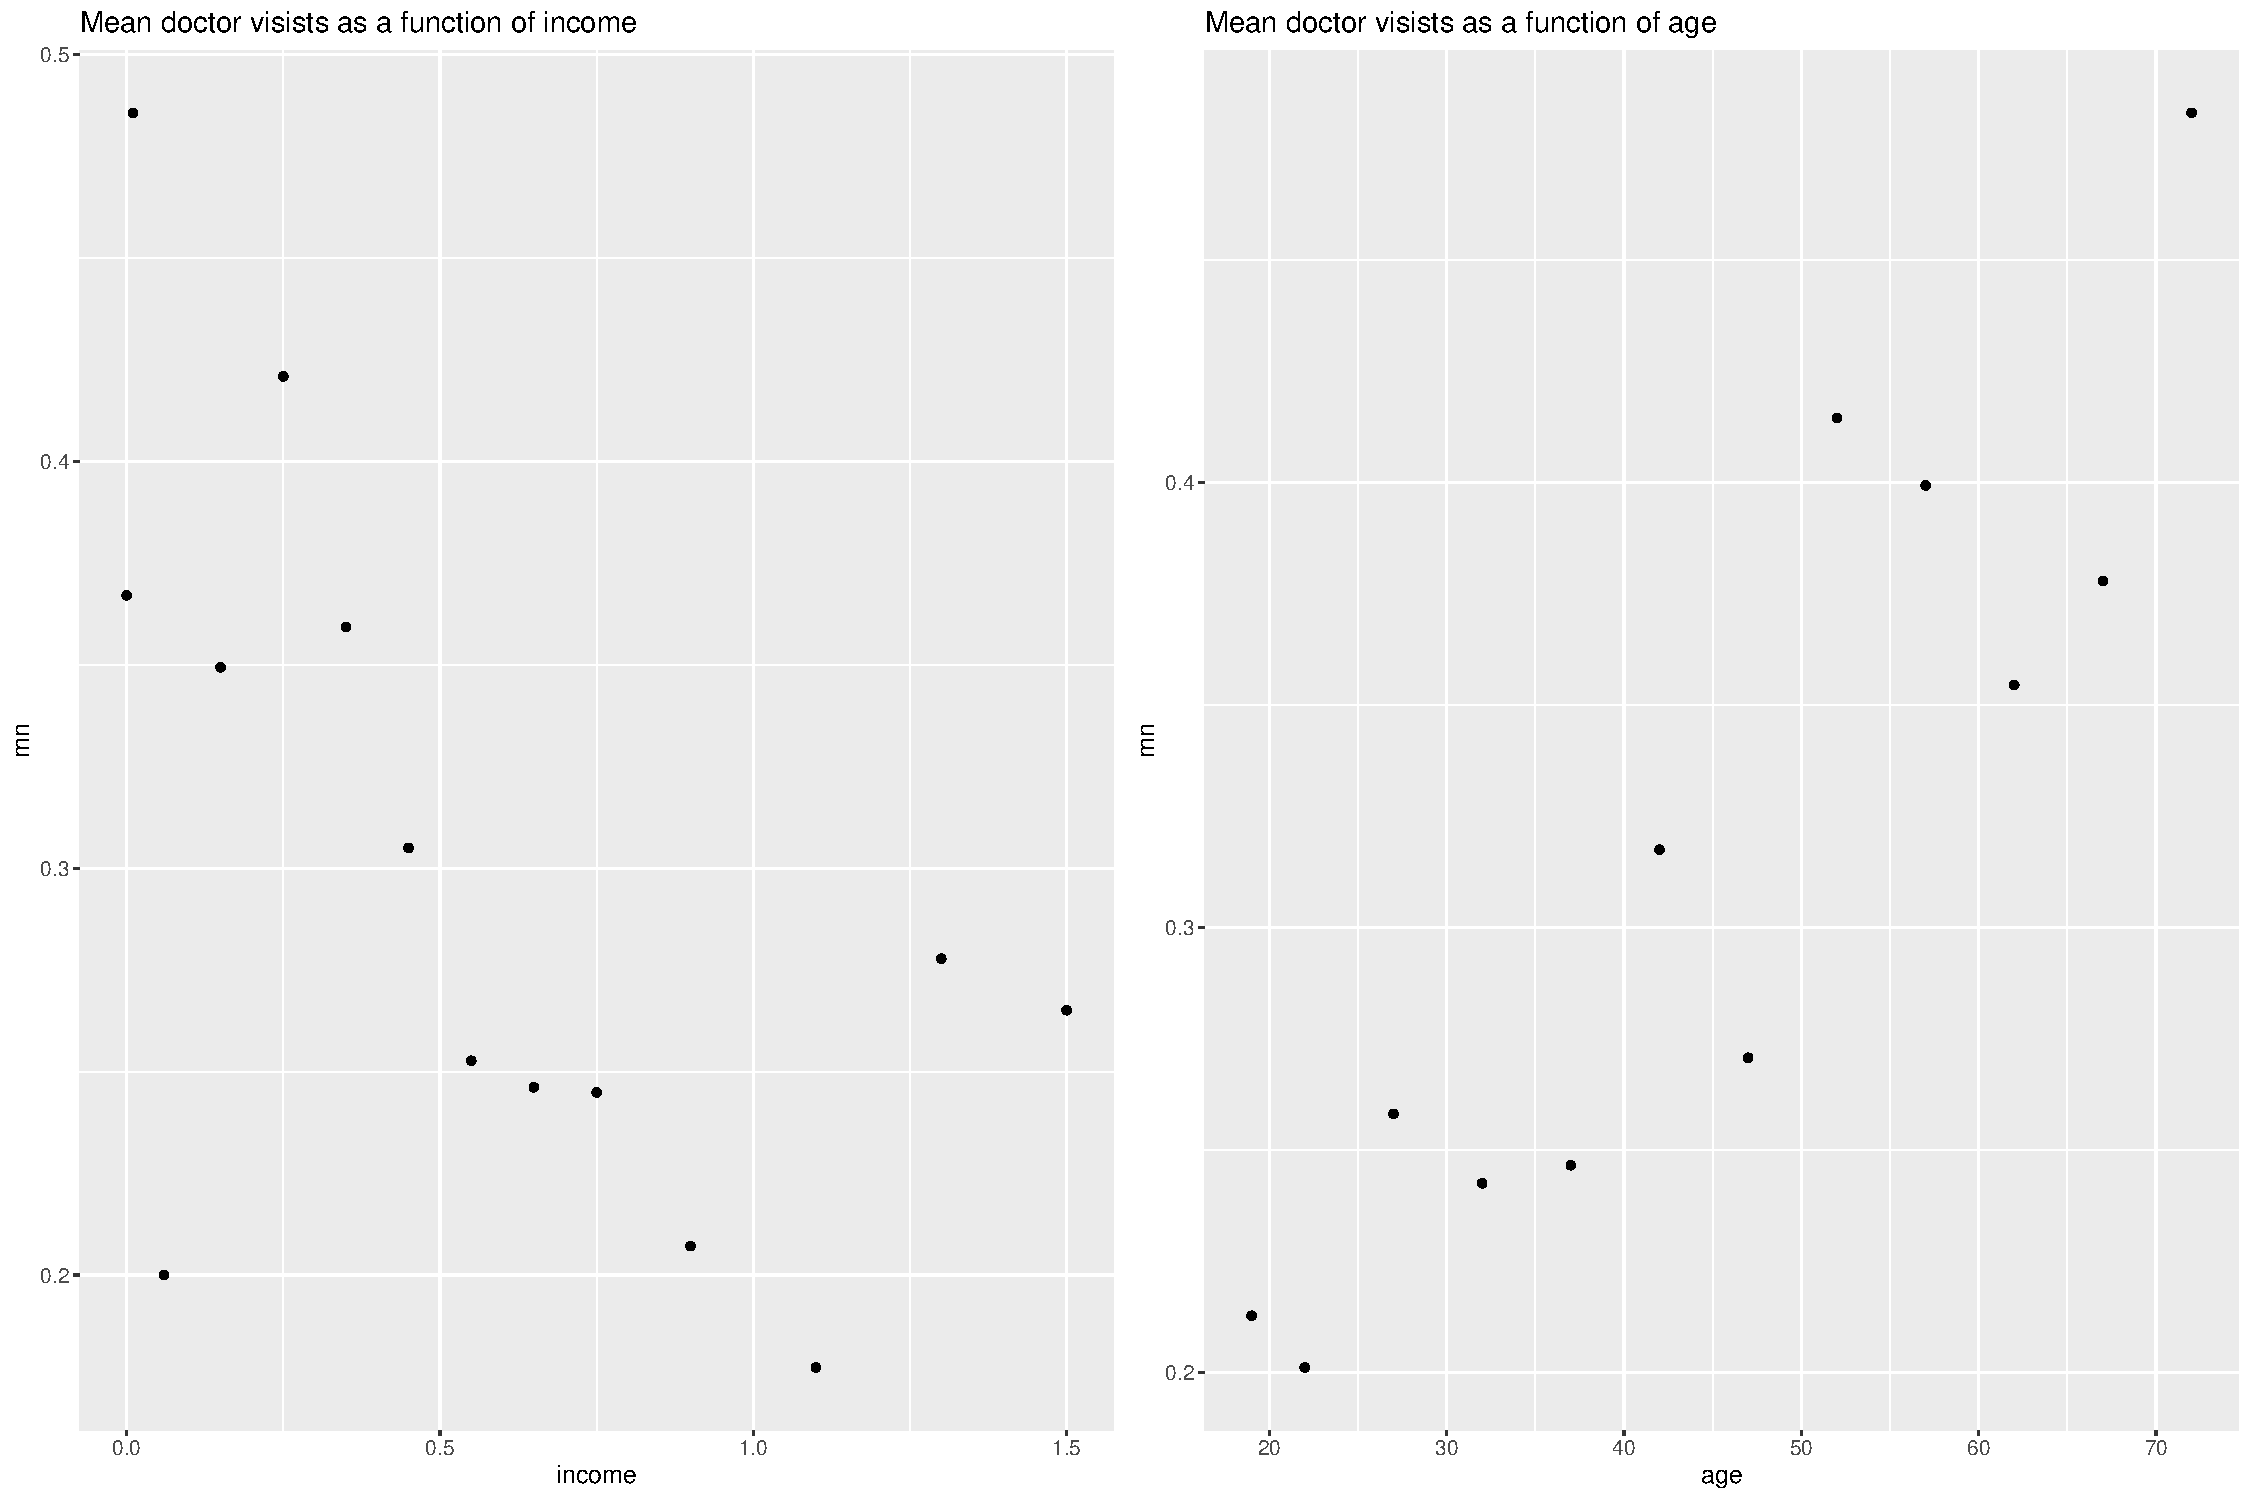
\includegraphics{../plots/mean_vs_income_and_age.pdf}
	\caption{Mean doctor visits as a function of income (left) and age (right)}
		\label{fig:scatter_income_and_age}
\end{figure}

\begin{figure}[h]
	\centering
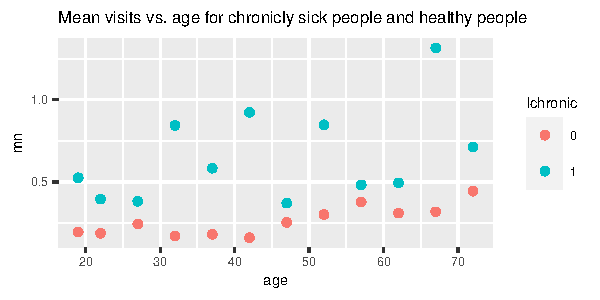
\includegraphics{../plots/mean_vs_age_and_chronic.pdf}

\caption{Mean doctor visits as a function of age for responses of chronically ill and healthy people}
\label{fig:scatter_age_and_chronic}
\end{figure}

One feature of $\mathbf{x}$ we have not analyzed yet is $x^{(c)}$, the binary indicator if the respondent has a chronic condition limiting activity. For this, we refer to figure \ref{fig:scatter_age_and_chronic}.  That plot shows the mean number of doctor visits as a function of respondent age, split by the value of $x^{(c)}$. From that plot, we may hypothesize that having a chronic disease increases the number of doctor visits. This also makes sense intuitively, as those patients need regularly scheduled check-ups or procedures.



\section{Modelling of the Relationship}
In the assignment, we were asked to develop a Poisson model with canonical link function. Thus, the relationship of $y_i$ and $\mathbf{x_i}$ is:
\begin{align}
& y_i \sim \text{Poisson}(\lambda_i) \\
&\lambda_i = \exp(\mathbf{x_i}^T\beta)
    \label{eq:model}
\end{align}
Since for the Poisson model we have $\mu = \lambda$, we see that the canonical link function in this case is $g(\mu) = \log(\mu)$.

The assignment further asks us to only consider the interaction term of the gender feature, $x^{(g)}$ with the other features of $\mathbf{x}$.

The model with all allowed interaction terms can be created in \texttt{R} with the following command:

\begin{verbatim}
glm(visits ~ . + gender*., data = df, family = poisson(link = log))
\end{verbatim}

After fitting this simple model, we analyze the z scores for the different coefficients of $\hat{\beta}$. The z values for many coefficients are suggesting that it is quite likely that they are zero. Hence, we will use a backwards AIC search to set certain estimates $\hat{\beta}_j$ to zero if that helps us reduce the AIC of the model.  This will be conducted with the \texttt{stepAIC} method from the \texttt{R MASS} package.

The backwards feature elimination found that the interaction terms of the gender with the income, the chronic disease indicator, and the categorical variable for the type of insurance should be removed.

In table \ref{tab:backwards_elimination}, we show the AIC, Deviance and the generalized $R^2$ metric as defined by Cameron and Windmeijer (1997). The analysis nicely shows how the removal of the three interaction terms (and 5 coefficients in $\hat{\beta}$ reduced the AIC while slightly increasing the Deviance and $R^2$ metric of the model, as expected. Note that we still chose the model with higher Deviance, because our model selection criterion is the AIC. A low AIC is desirable in our setting because we want to interpret the model at the end, hence we must strike a good balance between maximizing the likelihood and keeping the number of parameters, $p$, manageable.

\begin{table}[h]
    \centering
    \begin{tabular}{|c|c|c|c|}
    \hline
    Model & AIC & Deviance & $R^2$\\
    \hline
    Baseline Model with all features ($p=14$) &  7631.499 & 5271.931 & 0.644\\
    After backwards feature elimination ($p=9$) & 7624.555 & 5274.988  & 0.639\\
        \hline
        
    \end{tabular}
    \caption{Table of model diagnostics for the full model and the reduced model}
    \label{tab:backwards_elimination}
\end{table}

Now that we have the hypothesis that five parameters of the initial $\hat{\beta}$ may be $0$, we can construct a hypothesis test to confirm or disprove it. For this, we refer to section 4.4.3 of the lecture notes and use that, for $r<p$ we have
\begin{equation}
D^{(r)}(y) - D^{(p)}(y) \sim \chi^2_{(p-r)}
\end{equation}
Now, the difference in the deviances turns out to be $3.06$, and the difference in number of parameters is $5$. Hence, we have that $\mathbb{P}( \chi^2_{5} > 3.06) = 0.691$. Hence we can accept our hypothesis and move on with the model with the smaller number of parameters.

\section{Assessing model fit}
The most straightforward way to assess the model fit is to look at the scaled deviance of the model, $D(y)$. When the model is well fit, we expect $D(Y) \sim \chi^2_{(n-p)}$. With $D(y) = 5275, n = 5190$, and $p=9$, we have $\mathbb{P}( \chi^2_{5181} > 5275) = 0.178$. Although this is quite large, we can still accept this model at the $5\%$ acceptance limit. Also note, that for this data we do not expect the $\chi^2$ approximation for $D(y)$ to be perfect, since we have small counts in the Poisson.

One could also look at the standardized deviance and Pearson residuals. However, as discusses in the lectures, those residuals are not expected to be standard normals, although they should have unit variance.

We thus compute the standardized deviance residuals with the \texttt{R} command \texttt{rstandard} and find that the variance of those residuals is, in fact, $0.92$. Hence, the variance of the residuals is in the expected range.

\section{Model Interpretation}

We list all parameter estimates, their confidence intervals and means ratios in table \ref{tab:estimates}. Going back to equation \ref{eq:model}, the linear predictor has the form
\begin{align}
\eta_i &= \beta_0  +  \beta_2 x^{(i)} + \beta_3 \mathbbm{1}\{x^{(g)} = \text{"female"}\}     +\beta_4\mathbbm{1}\{x^{(c)} = 1\}   + 
 \beta_5\mathbbm{1}\{x^{(t)} = \text{"private"}\}    \\
 &+  \beta_6\mathbbm{1}\{x^{(t)} = \text{"freepoor"}\}  + \beta_7 \mathbbm{1}\{x^{(t)} = \text{"freerepat"}\}  \\
&+   x^{(a)}(\beta_8 \mathbbm{1}\{x^{(g)} = \text{"female"} \} + \beta_1)
\end{align}

\input{../report/estimates.txt}

The interested reader may refer to table \ref{tab:estimates} for all estimates and confidence intervals. We will focus on the estimates corresponding to the age, income, and chronic disease status of the respondents.

Looking at the confidence intervals of the estimates, it is striking that the parameters for the indicator that a respondent is female, and the parameter for the indicator that a respondent has free government healthcare due to poverty have the highest standard errors. That may indicate that the data has not a lot of information on the effect of those features.

Coming back to the interpretation of confidence intervals, we can say that, e.g. for $\beta_1$, the coefficient for the age of male respondents, upon repeating the same sampling from the population, the true parameter $\beta_1$ will be in 95\% of the confidence intervals.

Now, we shall look at the means ratio. If the means ratio for one parameter $\beta_j$ is $M^j$, then an increase of one unit in the variable $x_i^{(j)}$ means the expected number of doctor visits for a sample will be multiplied by  $M^j$. For example, the means ratio for the chronic disease state is $2.045$. This means that the expected number of doctor visits doubles if a respondent has the chronic disease! Similarly, the effect of the different insurances on the number of doctor visits can be nicely explained with the Means ratio. Compared with people with normal insurance, the expected number of doctor visits is 10\% higher for privately insured people, 36\% lower for people with free insurance due to poverty, and 13\% higher for people with free insurance due to veteran status. The means ratio also helps interpreting the influence of income on the expected number of doctor visits: An increase in income of ten thousand dollars will reduce the expected number of doctor visits by about 25\%

We also see that the means ratio for the age is $1.016$ for a male respondent. So, for an increase of 10 years in the respondent's age, the expected number of doctor visits will be multiplied by $1.016^{10} = 1.17$, i.e., it will increase by about 17\%. 

The influence of the age is slightly different for females compared to males. Let's define $\beta_a = \beta_8 + \beta_1$, the coefficient for the age variable, $x^{(a)}$ of females. Then, the approximate variance of that estimate is:
\begin{equation}
\widehat{var}(\hat{\beta}_a) = \widehat{var}(\hat{\beta}_8) + \widehat{var}(\hat{\beta}_1) + 2 \widehat{Cov}(\hat{\beta}_8, \hat{\beta}_1)
\end{equation}
Further, we can get the odds for an age increase of a female respodnent:
\begin{equation}
M_a = \exp(\beta_a) = \exp(\beta_8 + \beta_1)
\end{equation}
With all of this, we find the following numeric values:
\begin{table}[h]
    \centering
    \begin{tabular}{|c|c|c|c|c|c|}
    \hline
         index & beta\_i & Estimate & CI.Estimate & means ratio & CI.Means.Ratio\\
	\midrule
         Age (for women)& $\beta_a $ & 0.0048& [0.0029, 0.0066] & 1.0048 &[1.0029, 1.0066] \\
        \hline
    \end{tabular}
    \caption{Values for the age of a female}
    \label{tab:femal_age}
\end{table}

So, we see that the effect of age is almost negligible for women. For a ten year increase in the age, women are expected to go $1.0048^10 = 1.05$ times more often to the doctor. Hence, the increase for 10 years is 5\% for women compared to 17\% for men.

\section{Estimating the dispersion parameter}
In the lecture notes, we saw that 
\begin{equation}
\widehat{\phi} = \frac{1}{n-p} \sum_{i=1}^n \frac{(y_i- \hat{\mu}_i)^2}{V(\hat{\mu}_i)} = \frac{1}{n-p} \sum_{i=1}^n r_{P;i}^2
\end{equation}
Where $r_{P;i}$ is the (non-standardized) Pearson residual for sample $i$. Computing this in \texttt{R} yields an estimate of $\hat{\phi} = 1.992$. However, the real value for $\phi$ is $1$ in the Poisson model. Hence we should question whether the Poisson model, or the canonical link function, was actually a good choice in the first place.  

% TODO variables and z values

\end{document}
